\chapter{Proceso Paralelo e Interbloqueo}

Un concepto clave en los sistemas operativos es la aplicación de técnicas y algoritmos que optimizan la eficiencia de sus componentes, proporcionando al usuario el máximo rendimiento posible en un sistema informático. La evolución constante de las capacidades del hardware ha permitido la creación de equipos más potentes, capaces de realizar tareas en menos tiempo. Para gestionar de manera eficiente estas capacidades, las técnicas y algoritmos deben ser capaces de manejar adecuadamente las solicitudes de los procesos, tanto en el uso de dispositivos de entrada/salida como en el tiempo de procesador. Con el avance del hardware, estas solicitudes se han multiplicado, haciendo más necesario que nunca un control eficiente de los recursos.

\textbf{La analogía de los 5 filósofos}

Imaginemos cinco filósofos sentados alrededor de una mesa, cada uno con un plato de comida y un palillo a su derecha. Para comer, cada filósofo necesita dos palillos, lo que implica que deben compartir los palillos con sus vecinos. Si todos intentan comer al mismo tiempo, ninguno puede hacerlo, ya que falta un palillo para cada uno. Este escenario refleja los desafíos de la competencia entre procesos y la necesidad de coordinación para acceder a recursos compartidos.

\begin{figure}[H] \centering 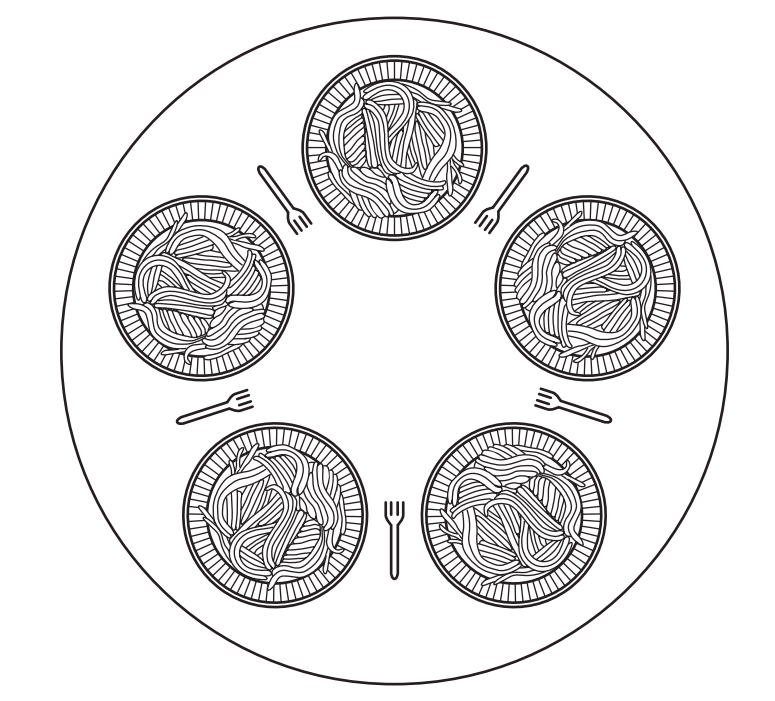
\includegraphics[width=0.8\linewidth]{Imagenes/los5filosofos.png} \caption{El problema representa los desafíos que tienen los sistemas operativos para gestionar los procesos.} \end{figure}

\section{Proceso Paralelo}

El proceso paralelo consiste en la ejecución simultánea de múltiples procesos en un sistema operativo. Su principal objetivo es mejorar el rendimiento y la eficiencia del sistema al distribuir tareas entre varios procesadores o núcleos, permitiendo que el sistema ejecute varias tareas a la vez. En sistemas con múltiples procesadores, el paralelismo es real; en sistemas de un solo procesador, el paralelismo es aparente y depende de técnicas como la multiprogramación.

El proceso paralelo es esencial para reducir tiempos de espera, aumentar la capacidad de respuesta del sistema y mejorar la experiencia del usuario. Se utiliza en aplicaciones que manejan grandes volúmenes de datos, simulaciones científicas, o en servidores que requieren alta capacidad de procesamiento.

\subsection{Exclusión Mutua}

La exclusión mutua es un principio fundamental que asegura que solo un proceso a la vez pueda acceder a un recurso compartido. Esto es importante para evitar que múltiples procesos intenten modificar el mismo recurso simultáneamente, lo que podría causar errores o corrupción de datos.

Un ejemplo claro de la necesidad de exclusión mutua ocurre en un sistema bancario. Imagina que dos cajeros automáticos, ubicados en diferentes lugares, intentan acceder al saldo de la misma cuenta bancaria para procesar retiros simultáneamente. Sin un mecanismo de exclusión mutua, ambos cajeros podrían retirar dinero al mismo tiempo, lo que provocaría que el saldo sea incorrecto o incluso que se retire más dinero del disponible. La exclusión mutua garantiza que solo uno de los cajeros pueda acceder a la cuenta en un momento dado, bloqueando temporalmente el acceso del otro hasta que la operación haya finalizado. Esto asegura que las transacciones se realicen de manera segura y consistente.

\begin{figure}[H] \centering 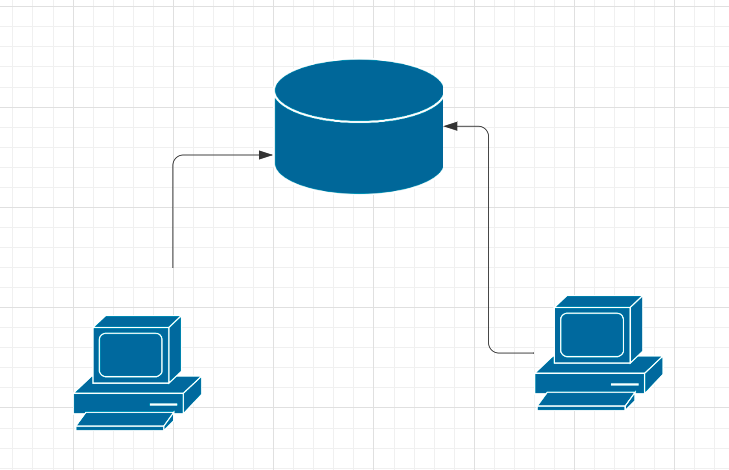
\includegraphics[width=0.8\linewidth]{Imagenes/exclusion.png} \caption{La exclusión mutua asegura que los recursos compartidos sean utilizados de manera controlada.} \end{figure}

\subsection{Sincronización}

La sincronización es el mecanismo que coordina la ejecución de múltiples procesos para asegurar que accedan a los recursos compartidos de manera ordenada y controlada. Sin la sincronización adecuada, los procesos podrían acceder a los recursos de forma desorganizada, lo que podría generar conflictos, errores o resultados inesperados.

Volviendo al ejemplo de los cajeros automáticos, la sincronización asegura que los procesos que intentan acceder al saldo de una cuenta se coordinen correctamente. Aunque la exclusión mutua previene que ambos cajeros accedan simultáneamente al saldo, la sincronización es lo que garantiza que los cajeros se coordinen y esperen su turno de manera ordenada. De esta forma, cuando un cajero completa su transacción, el otro puede acceder al saldo sin causar inconsistencias en la cuenta.

\subsubsection{Importancia de la Sincronización} \begin{itemize} \item \textbf{Integridad de Datos:} Previene condiciones de carrera, donde los resultados dependen del orden no controlado de ejecución de los procesos. \item \textbf{Eficiencia:} Permite que los procesos avancen de manera ordenada y se eviten bloqueos innecesarios, garantizando un uso óptimo de los recursos. \item \textbf{Estabilidad del Sistema:} Asegura que los procesos concurrentes no generen errores o comportamientos inesperados en el sistema operativo. \end{itemize}

\newpage

\section{Interbloqueo en Sistemas Operativos}

El \textbf{interbloqueo} es una situación en sistemas operativos donde un conjunto de procesos se encuentra en un estado de espera permanente, ya que cada uno está esperando que ocurra un evento que solo puede ser provocado por otro proceso del conjunto. Ninguno de los procesos puede avanzar porque todos dependen mutuamente de recursos que están siendo utilizados por los demás, entrando así en una espera indefinida.

\textbf{Ejemplo Ilustrativo}

Imagine una carretera de doble sentido que, en cierto punto, se estrecha debido a un puente que solo permite el paso de vehículos en un solo sentido. Si un vehículo entra desde cada extremo al mismo tiempo, ambos se encontrarán en el centro del puente. Ninguno puede avanzar porque el camino está bloqueado por el otro, y retroceder podría ser difícil o imposible. Ambos conductores esperan que el otro ceda el paso, pero si ninguno lo hace, se genera un \textbf{interbloqueo} y ambos vehículos quedan inmovilizados.

\begin{figure}[H] \centering 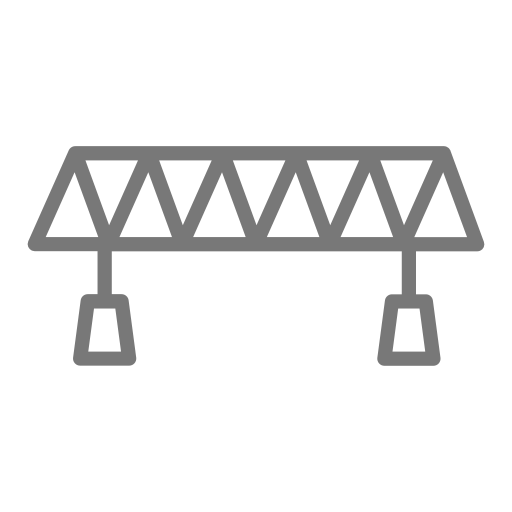
\includegraphics[width=0.6\linewidth]{Imagenes/puente.png} \caption{Un puente de una sola vía, representa al interbloqueo, cuando dos vehículos en dirección opuesta tratan de cruzar al mismo tiempo.} \end{figure}

Este ejemplo refleja cómo en un sistema operativo, procesos pueden quedar bloqueados esperando recursos que están siendo utilizados por otros procesos, sin posibilidad de que ninguno avance.

\subsection{Recursos en Sistemas Operativos}


En sistemas operativos, un \textbf{recurso} es cualquier componente de hardware o software necesario para que un proceso pueda ejecutar sus tareas. Los recursos pueden clasificarse en:
\textbf{Hardware} (CPU, Memoria, Dispositivos E/S), y \textbf{Software} (Archivos, registros). 

Estos  tienen definido un ciclo de uso, como se detalla a continuación:


\begin{enumerate}
	\item \textbf{Solicitud}: El proceso pide el recurso que necesita para continuar su ejecución.
	\item \textbf{Asignación/Utilización}: Si el recurso está disponible, el sistema operativo lo asigna al proceso, que entonces lo utiliza para realizar su tarea.
	\item \textbf{Liberación}: Una vez que el proceso ha terminado de usar el recurso, lo libera para que otros procesos puedan utilizarlo.
\end{enumerate}

Es fundamental que este ciclo se gestione de manera eficiente para evitar conflictos y asegurar que los recursos se utilizan de forma óptima.

\subsection{Modelo de Interbloqueo (Abrazo Mortal)}

El \textbf{interbloqueo}, también conocido como ``abrazo mortal'',  se produce cuando un conjunto de procesos compite por recursos y terminan bloqueándose mutuamente. Esto ocurre porque cada proceso espera que ocurra un evento (como la liberación de un recurso) que solo puede ser provocado por otro proceso dentro del mismo conjunto.

\subsubsection{¿En Qué Consiste?}

\begin{itemize}
	\item \textbf{Dependencia Circular}: Cada proceso en el conjunto está esperando por un recurso que está siendo retenido por otro proceso. Esta cadena de dependencias forma un ciclo cerrado.
	\item \textbf{Espera Indefinida}: Ninguno de los procesos puede avanzar porque están esperando indefinidamente que los recursos sean liberados, pero esto no ocurre porque todos están bloqueados.
\end{itemize}

\textbf{Ejemplo Detallado}:

Supongamos que tenemos dos procesos, \textbf{P1} y \textbf{P2}, y dos recursos, \textbf{R1} y \textbf{R2}.

\begin{itemize}
	\item \textbf{P1} tiene asignado \textbf{R1} y solicita \textbf{R2}.
	\item \textbf{P2} tiene asignado \textbf{R2} y solicita \textbf{R1}.
\end{itemize}

Ambos procesos esperan indefinidamente porque ninguno liberará su recurso hasta obtener el otro. Este es un ciclo de espera circular que provoca un interbloqueo.

\subsection{Postergación Indefinida (Starvation)}

La \textbf{postergación indefinida} ocurre cuando un proceso espera por un recurso durante un tiempo extremadamente largo o potencialmente infinito, sin garantías de que lo obtendrá. Esto suele deberse a políticas de planificación que no aseguran equidad entre los procesos.

\subsubsection{Relación con la Planificación}

\begin{itemize}
	\item \textbf{Prioridades Desbalanceadas}: Si los procesos de alta prioridad siguen llegando al sistema, los de baja prioridad pueden quedar postergados indefinidamente.
	\item \textbf{Ausencia de Mecanismos de Equidad}: Sin técnicas como la planificación circular (round-robin) o la asignación de cuotas de tiempo, algunos procesos pueden no recibir nunca los recursos que necesitan.
\end{itemize}

Aunque la postergación indefinida y el interbloqueo pueden parecer similares porque ambos resultan en procesos que no avanzan, son problemas distintos. En la postergación indefinida, no hay dependencia cíclica de recursos; es un problema de planificación y asignación de recursos.

\subsection{Condiciones para el Interbloqueo}

Para que ocurra un interbloqueo, deben cumplirse simultáneamente las siguientes cuatro condiciones:

\begin{enumerate}
	\item \textbf{Exclusión Mutua}: Mecanismo por el cual se garantiza que solo un proceso a la vez pueda acceder a un recurso. Por ejemplo, una impresora.
	\item \textbf{Posesión y Espera}: Un proceso está sosteniendo al menos un recurso y está esperando para obtener recursos adicionales que están siendo sostenidos por otros procesos. Por ejemplo, un proceso tiene una impresora y espera por un escáner que está en uso.
	\item \textbf{No Apropiación}: Los recursos no pueden ser retirados forzosamente de los procesos que los poseen; solo pueden ser liberados voluntariamente. Esto significa que si un proceso sostiene un recurso y otro proceso necesita ese mismo recurso, el sistema no puede forzar al proceso que lo tiene a liberar dicho recurso. 
	\item \textbf{Espera Circular}: Existe un conjunto de procesos \(\{P_1, P_2, \ldots, P_n\}\) tal que \(P_1\) está esperando un recurso sostenido por \(P_2\), \(P_2\) está esperando un recurso sostenido por \(P_3\), \ldots, y \(P_n\) está esperando un recurso sostenido por \(P_1\).
\end{enumerate}

Si todas estas condiciones se cumplen al mismo tiempo, el sistema está en un estado de interbloqueo.

\subsection{Tratamiento del Interbloqueo}

Existen varias estrategias para manejar los interbloqueos en sistemas operativos:

\subsubsection{1. Ignorar el Problema}

\begin{itemize}
	\item \textbf{Política del ``Ostrich''}: El sistema asume que los interbloqueos son tan poco frecuentes que no vale la pena invertir en mecanismos para prevenirlos o resolverlos.
	\item \textbf{Ventajas}:
	\begin{itemize}
		\item Simplicidad en el diseño del sistema operativo.
		\item Ahorro de recursos y tiempo de procesamiento.
	\end{itemize}
	\item \textbf{Desventajas}:
	\begin{itemize}
		\item Riesgo de que el sistema se congele si ocurre un interbloqueo.
		\item No es adecuado para sistemas donde la confiabilidad es crítica.
	\end{itemize}
\end{itemize}

\subsubsection{2. Prevención del Interbloqueo}

Esta estrategia modifica el sistema para garantizar que al menos una de las condiciones necesarias para el interbloqueo no pueda ocurrir.

\begin{itemize}
	\item \textbf{Eliminar la Exclusión Mutua}:
	\begin{itemize}
		\item Difícil, ya que algunos recursos son inherentemente no compartibles.
		\item Solución: Diseñar recursos virtuales o utilizar mecanismos de spooling (por ejemplo, en impresoras).
	\end{itemize}
	\item \textbf{Evitar la Posesión y Espera}:
	\begin{itemize}
		\item Requerir que los procesos soliciten todos los recursos que necesitan al inicio.
		\item Desventaja: Ineficiente y puede conducir a la subutilización de recursos.
	\end{itemize}
	\item \textbf{Permitir la Apropiación}:
	\begin{itemize}
		\item Si un proceso necesita un recurso, el sistema puede quitarle el recurso a otro proceso.
		\item Implementado mediante mecanismos de suspensión y reanudación de procesos.
	\end{itemize}
	\item \textbf{Romper la Espera Circular}:
	\begin{itemize}
		\item Impone un orden jerárquico en la solicitud de recursos.
		\item Los procesos deben solicitar recursos en un orden predefinido.
	\end{itemize}
\end{itemize}



\subsubsection{4. Detección y Recuperación}

Permitir que el interbloqueo ocurra, pero tener mecanismos para detectarlo y recuperarse.

\begin{itemize}
	\item \textbf{Detección}:
	\begin{itemize}
		\item Implementar algoritmos que periódicamente verifican si el sistema está en un estado de interbloqueo.
		\item Buscan ciclos en el \textit{grafo de asignación de recursos}.
	\end{itemize}
	\item \textbf{Recuperación}:
	\begin{itemize}
		\item \textbf{Abortar Procesos}: Terminar uno o más procesos para romper el ciclo de espera.
		\begin{itemize}
			\item Criterios: Prioridad del proceso, tiempo de ejecución, recursos utilizados.
		\end{itemize}
		\item \textbf{Reclamo forzado	 de Recursos}: Forzar la liberación de recursos de ciertos procesos.
		\begin{itemize}
			\item Puede requerir la implementación de puntos de recuperación (checkpoints) para reiniciar procesos.
		\end{itemize}
	\end{itemize}
\end{itemize}




